\documentclass[a4paper,12pt]{article} 


\usepackage[T2A]{fontenc}			
\usepackage[utf8]{inputenc}			
\usepackage[english,russian]{babel}	

\usepackage{graphicx, scalerel}    
\usepackage{wrapfig}               
\usepackage[14pt]{extsizes}        
\usepackage[warn]{mathtext}       
\usepackage{indentfirst}      
\usepackage[margin = 25mm]{geometry}
\usepackage[table,xcdraw]{xcolor} 
\usepackage{amsmath,amsfonts,amssymb,amsthm,mathtools}
\usepackage{wasysym}                
\usepackage{upgreek}                
\usepackage{caption}
\usepackage{multirow}
\captionsetup{labelsep=period}
\usepackage[font=small,labelfont=bf]{caption}
\usepackage{gensymb}
\usepackage{icomma}

\usepackage[unicode, pdftex]{hyperref}
\usepackage{tikz}
\usetikzlibrary{positioning}
\usepackage{fancyhdr}
\pagestyle{fancy}
\setlength\fboxsep{3pt} % Отступ рамки \fbox{} от рисунка
\setlength\fboxrule{1pt} % Толщина линий рамки \fbox{}
\usepackage{tocloft}
\newcommand{\tocsection}[1]{\section*{#1} \addcontentsline{toc}{section}{#1}}
\newcommand{\tocsubsection}[1]{\subsection*{#1} \addcontentsline{toc}{subsection}{#1}}
\renewcommand{\cftsecleader}{\cftdotfill{\cftdotsep}}

\begin{document}
	\newcommand{\HRule}{\rule{\linewidth}{0.7mm}} % Defines a new command for the horizontal lines, change thickness here

\begin{center}
	\large\textbf{Московский Физико-Технический Институт}\\
	\large\textbf{(государственный университет)}
	
	\vfill
	
	
	
	\Large Лабораторная работа 5.1.2
	%----------------------------------------------------------------------------------------
	%	TITLE SECTION
	%----------------------------------------------------------------------------------------
	
	\HRule
	\\[0.4cm]
	{ \huge \bfseries Исследование эффекта Комптона}
	\\[0.4cm] % Title of your document
	\HRule
	\\[0.5cm]
	
	\ \\
	\textbf{\large Автор:} \\	
	\large Овсянников Михаил Б01-008\\
	\vfill
	\hspace*{-0.8 cm}
\includegraphics[width=100 pt]{./Include/frkt_logo.pdf}\\
	\large Долгопрудный, 2022
\end{center}

\thispagestyle{empty}

\newpage
\setcounter{page}{2}
\fancyfoot[c]{\thepage}
\fancyhead[L] {Лабораторная работа 5.1.2}
\fancyhead[R] {Исследование эффекта Комптона}

	\newpage
	
	\tableofcontents
	
	
	
	\newpage
	\textbf{Цель работы:} c помощью магнитного спектрометра исследовать энергетический спектр $\beta$-частиц при распаде ядер $^{137}$Cs и определить их максимальную энергию.

	
	
	\tocsection{Теоретические сведения}
	Бета-распадом называется самопроизвольное превращение ядер, при котором их массовое число не изменяется, а заряд увеличивается или уменьшается на единицу. Бета-активные ядра встречаются во всей области значений массового числа $A$, начиная от единицы (свободный нейтрон) и кончая самыми тяжелыми ядрами.	
	
	В данной работе мы будем иметь дело с электронным распадом
	
	\begin{equation*}
		_Z^A\text{X} \; \longrightarrow \;\; _{Z+1}^{\;\;\;\;\,A}\text{X} + e^- + \widetilde{\nu},
	\end{equation*}

	\noindent при котором кроме электрона испускается антинейтрино. Освобождающаяся при $\beta$-распаде энергия делится между электроном, антинейтрино и дочерним ядром, однако доля энергии, передаваемой ядру, исчезающе мала по сравнению с энергией, уносимой электроном и антинейтрино. Практически можно считать, что эти две частицы делят между собой всю освобождающуюся энергию. Поэтому электроны могут иметь любое значение энергии — от нулевой до некоторой максимальной, которая равна энергии, освобождающейся при $\beta$-распаде, являющейся важной физической величиной.
	
	Кинетическая энергия электрона $E$ связана с его импульсом обычным релятивистским соотношением
	\begin{equation}
		E = \sqrt{(pc)^2 + (mc^2)^2} - mc^2.
	\end{equation}

	\begin{wrapfigure}{r}{0.4\textwidth}
		\centering
		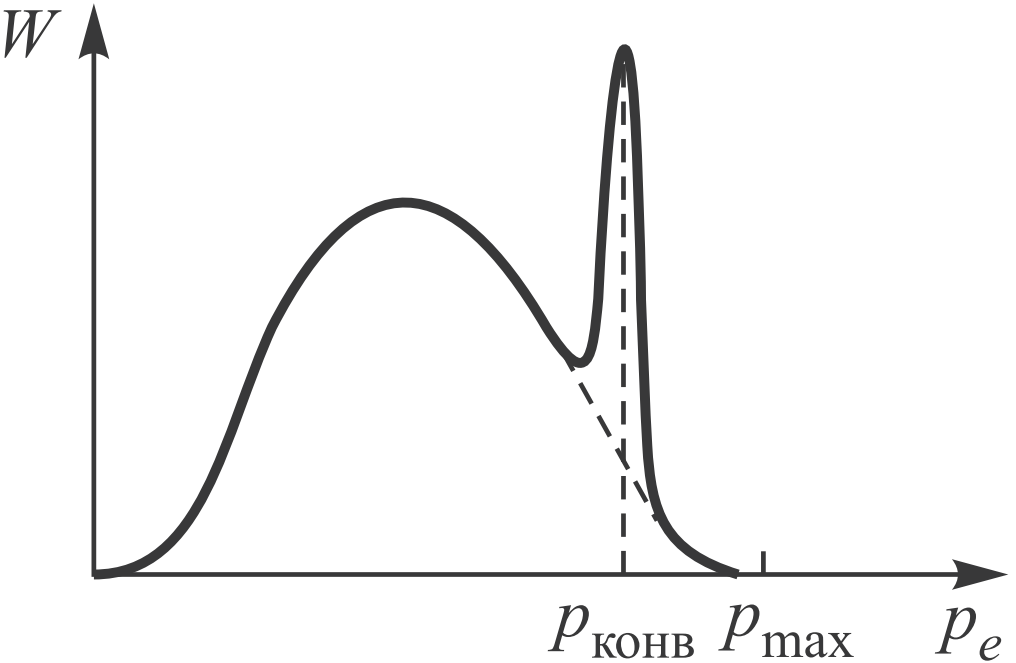
\includegraphics[width=1\linewidth]{Pictures/W(p)}
		\caption{Форма спектра $\beta$-частиц при разрешенных переходах}
		\label{BetaParticles_Spectre}
	\end{wrapfigure}

	В нерелятивистском приближении формула, выражающая форму $\beta$-спектра приобретает вид:
	\begin{equation}
		\frac{dN}{dE} = \sqrt{E}(E_e - E)^2,
		\label{BetaParticles_dNdE}
	\end{equation}

	\noindent где $E_e$ — максимальная энергия электрона.
	
	Выражение (\ref{BetaParticles_dNdE}) приводит к спектру, имеющему вид широкого колокола (см. рис. \ref{BetaParticles_Spectre}). Кривая плавно отходит от нуля и столь же плавно, по параболе, касается оси абсцисс в области максимальной энергии электронов $E_e$.
	
	
	Дочерние ядра, возникающие в результате $\beta$-распада, нередко оказываются возбужденными. Возбужденные ядра отдают свою энергию либо излучая $\gamma$-квант (энергия которого равна разности энергий начального и конечного уровней), либо передавая избыток энергии одному из электронов с внутренних оболочек атома. Излучаемые в таком процессе электроны имеют строго определенную энергию и называются конверсионными.

	Конверсия чаще всего происходит на оболочках $K$ или $L$. На спектре, представленном на рис. \ref{BetaParticles_Spectre}, видна монохроматическая линия, вызванная электронами конверсии. Ширина этой линии в нашем случае является чисто аппаратурной — по ней можно оценить разрешающую силу спектрометра.

	
	\tocsection{Экспериментальная установка}
	\begin{figure}[h!]
		\centering
		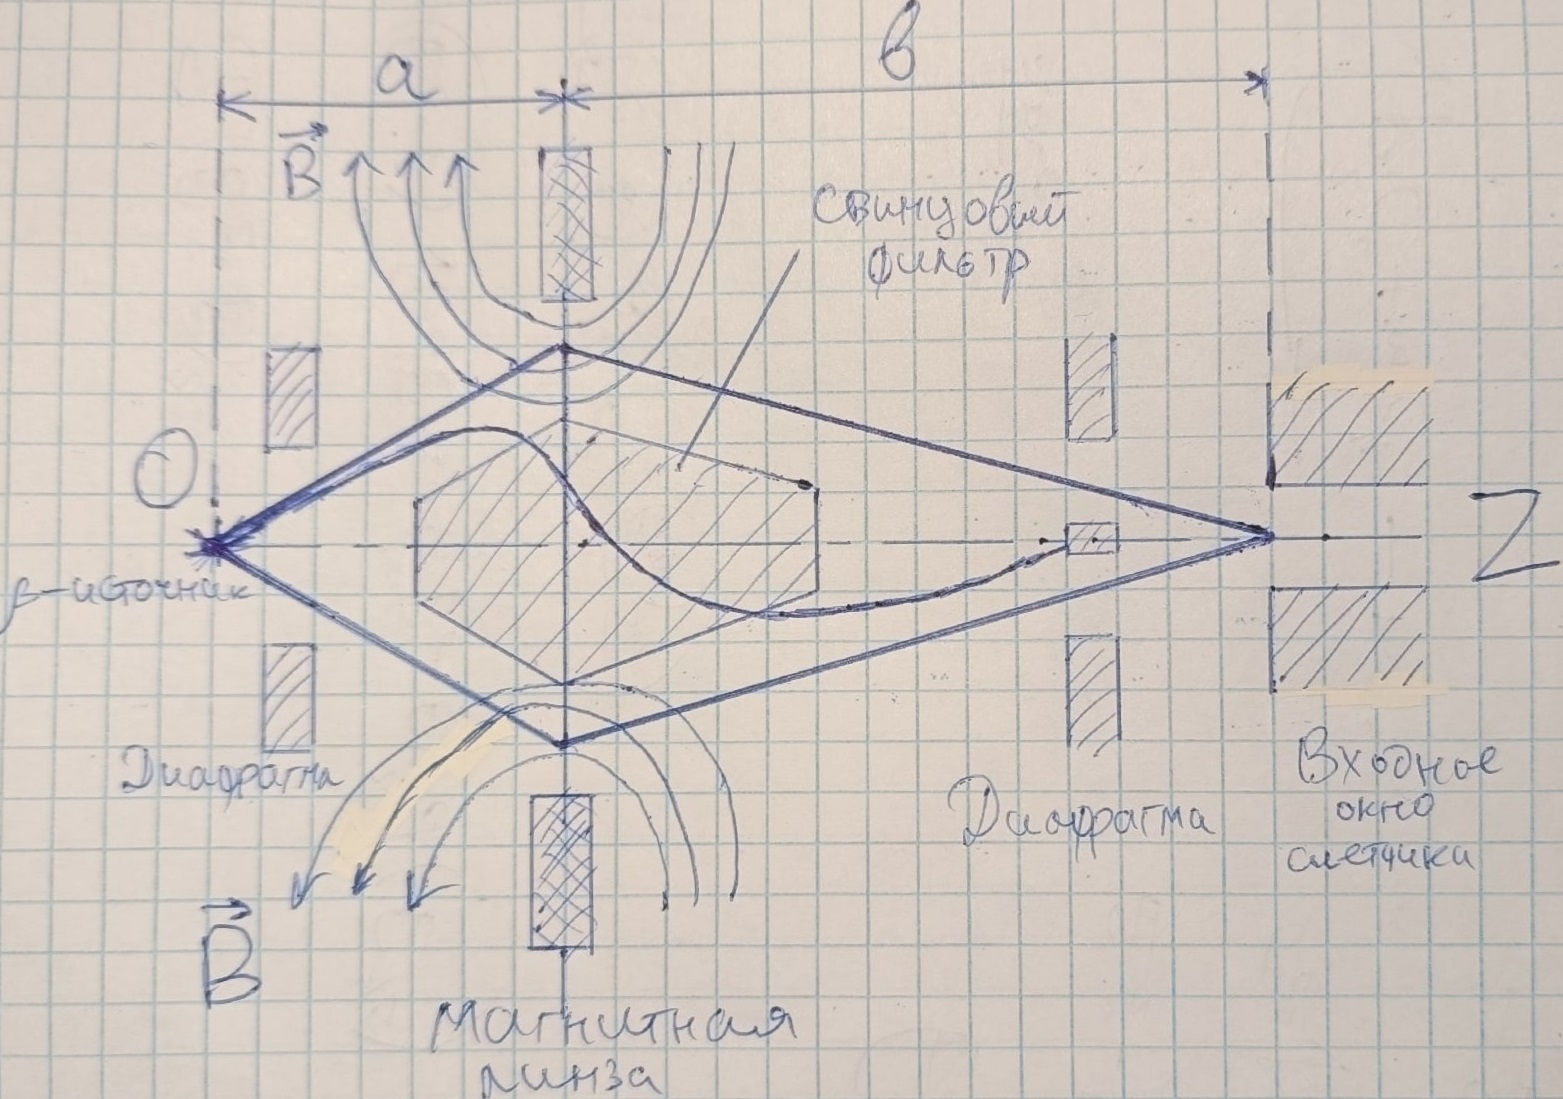
\includegraphics[width=\linewidth]{Pictures/Scheme}
		\caption{Схема $\beta$-спектрометра с короткой магнитной линзой}
		\label{BetaParticles_Scheme}
	\end{figure}

	Энергию $\beta$-частиц определяют с помощью $\beta$-спектрометров. В работе используется магнитный спектрометр с «короткой линзой». Электроны, испускаемые радиоактивным источником (рис. \ref{BetaParticles_Scheme}), попадают в магнитное поле катушки, ось которой параллельна оси $OZ$ (оси симметрии прибора). Траектории электронов в магнитном поле представляют собой схематически показанные на рисунке сложные спирали, сходящиеся за катушкой в фокусе, расположенном на оси $OZ$. В фокусе установлен детектор электронов. Чувствительным элементом сцинтилляционного счетчика является тонкий кристалл полистирола. При попадании электрона в кристалле возникает световая вспышка -- сцинтилляция, регистрируемая фотоумножителем.
	
	При заданной силе тока на входное окно счетчика фокусируются электроны с определенным импульсом. Электроны, обладающие другими значениями импульса, при этом не сфокусированы и в основном проходят мимо окна (штриховой луч). При изменении тока в катушке на счетчик последовательно фокусируются электроны с разными импульсами. Так как геометрия прибора в течение всего опыта остается неизменной, импульс сфокусированных электронов пропорционален величине тока $I$:
	\begin{equation}
		p_e = kI.
		\label{BetaParticles_pkI}
	\end{equation}


	Из-за конечных размеров источника, диафрагм и окна счетчика, а также вследствие аберраций при заданной величине фокусного расстояния на счетчик попадают электроны с импульсами, лежащими внутри некоторого интервала от $p_e - \Delta p_e/2$ до $p_e + \Delta p_e/2$. Величина $\Delta p_e$ -- ширина интервала импульсов, регистрируемых при заданном значении тока, -- называется разрешающей способностью $\beta$-спектрометра.
	
	Ширина интервала $\Delta p_e$, регистрируемого спектрометром, пропорциональна величине импульса.
	
	В результате попадания электронов в сцинтиллятор на выходе фотоумножителя появляются электрические импульсы, которые заносятся в память персонального компьютера и выводятся на экран монитора. Давление в спектрометре поддерживается на уровне около 0,1 Тор и измеряется термопарным вакуумметром. Лучший вакуум в приборе не нужен, поскольку уже при этом давлении потери энергии электронов малы и их рассеяние незначительно. Откачка осуществляется форвакуумным насосом. Магнитная линза питается постоянным током от выпрямителя. Высокое напряжение на ФЭУ или газоразрядный счетчик подается от стабилизированного выпрямителя.
	
	\tocsection{Ход работы}
	\begin{enumerate}
		\item Откачаем воздух из полости спектрометра.
		
		\item Включим формирователь импульсов, питание магнитной линзы и уменьшим ток через нее до нуля.
		
		\item Приступим к подробному измерению $\beta$-спектра. Результаты запишем в таблицу \ref{BetaParticles_ExpTable}.
		\begin{figure}[h!]
			\centering
			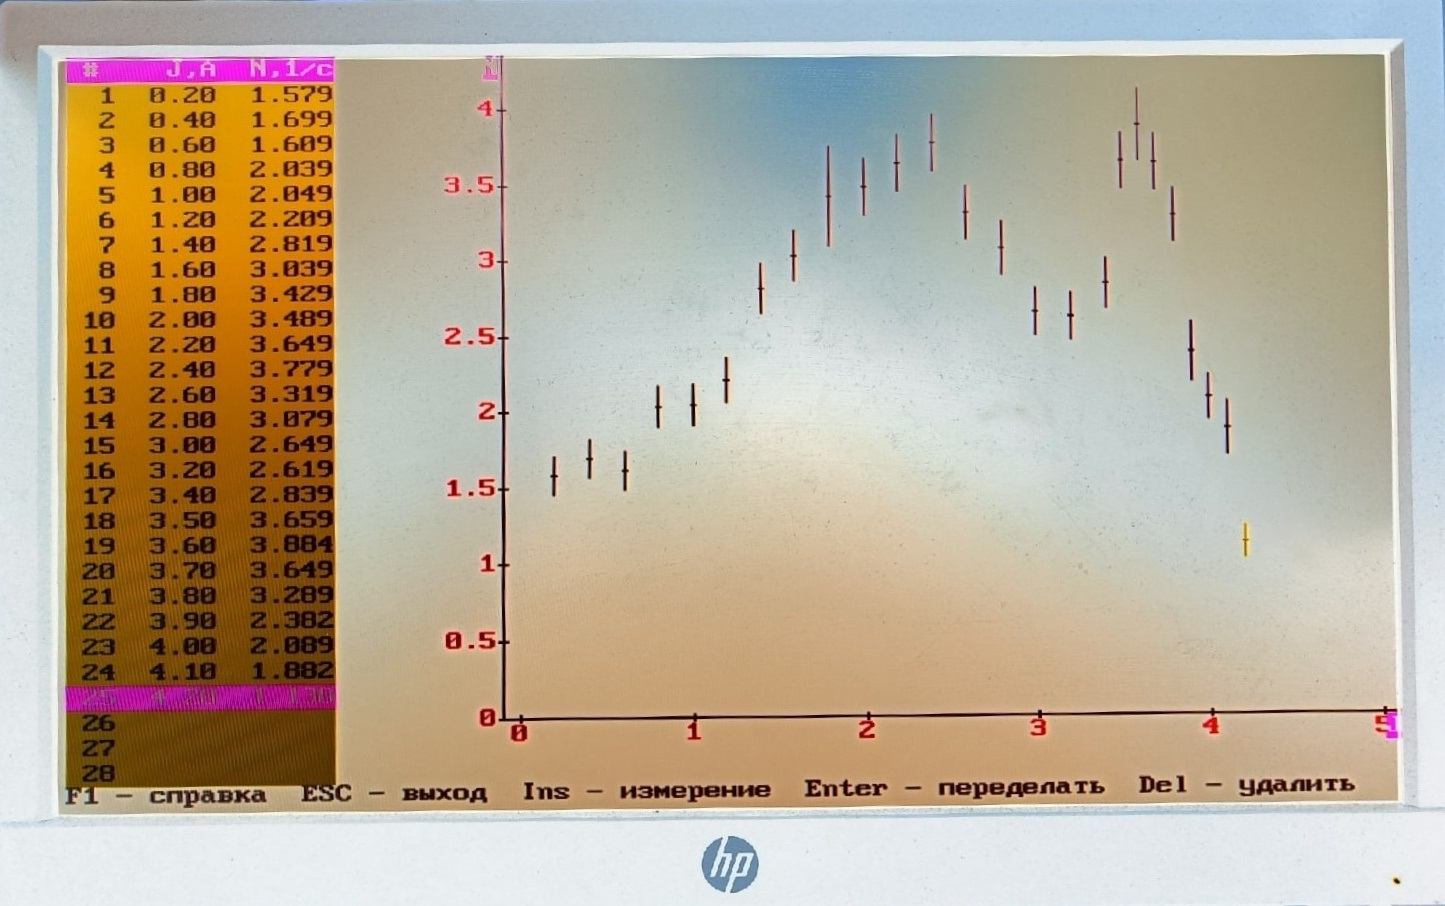
\includegraphics[width=0.9\linewidth]{Pictures/CompSpectreNeg}
			\caption{Картина спектра на компьютере}
		\end{figure}
	
		\begin{figure}[h!]
			\centering
			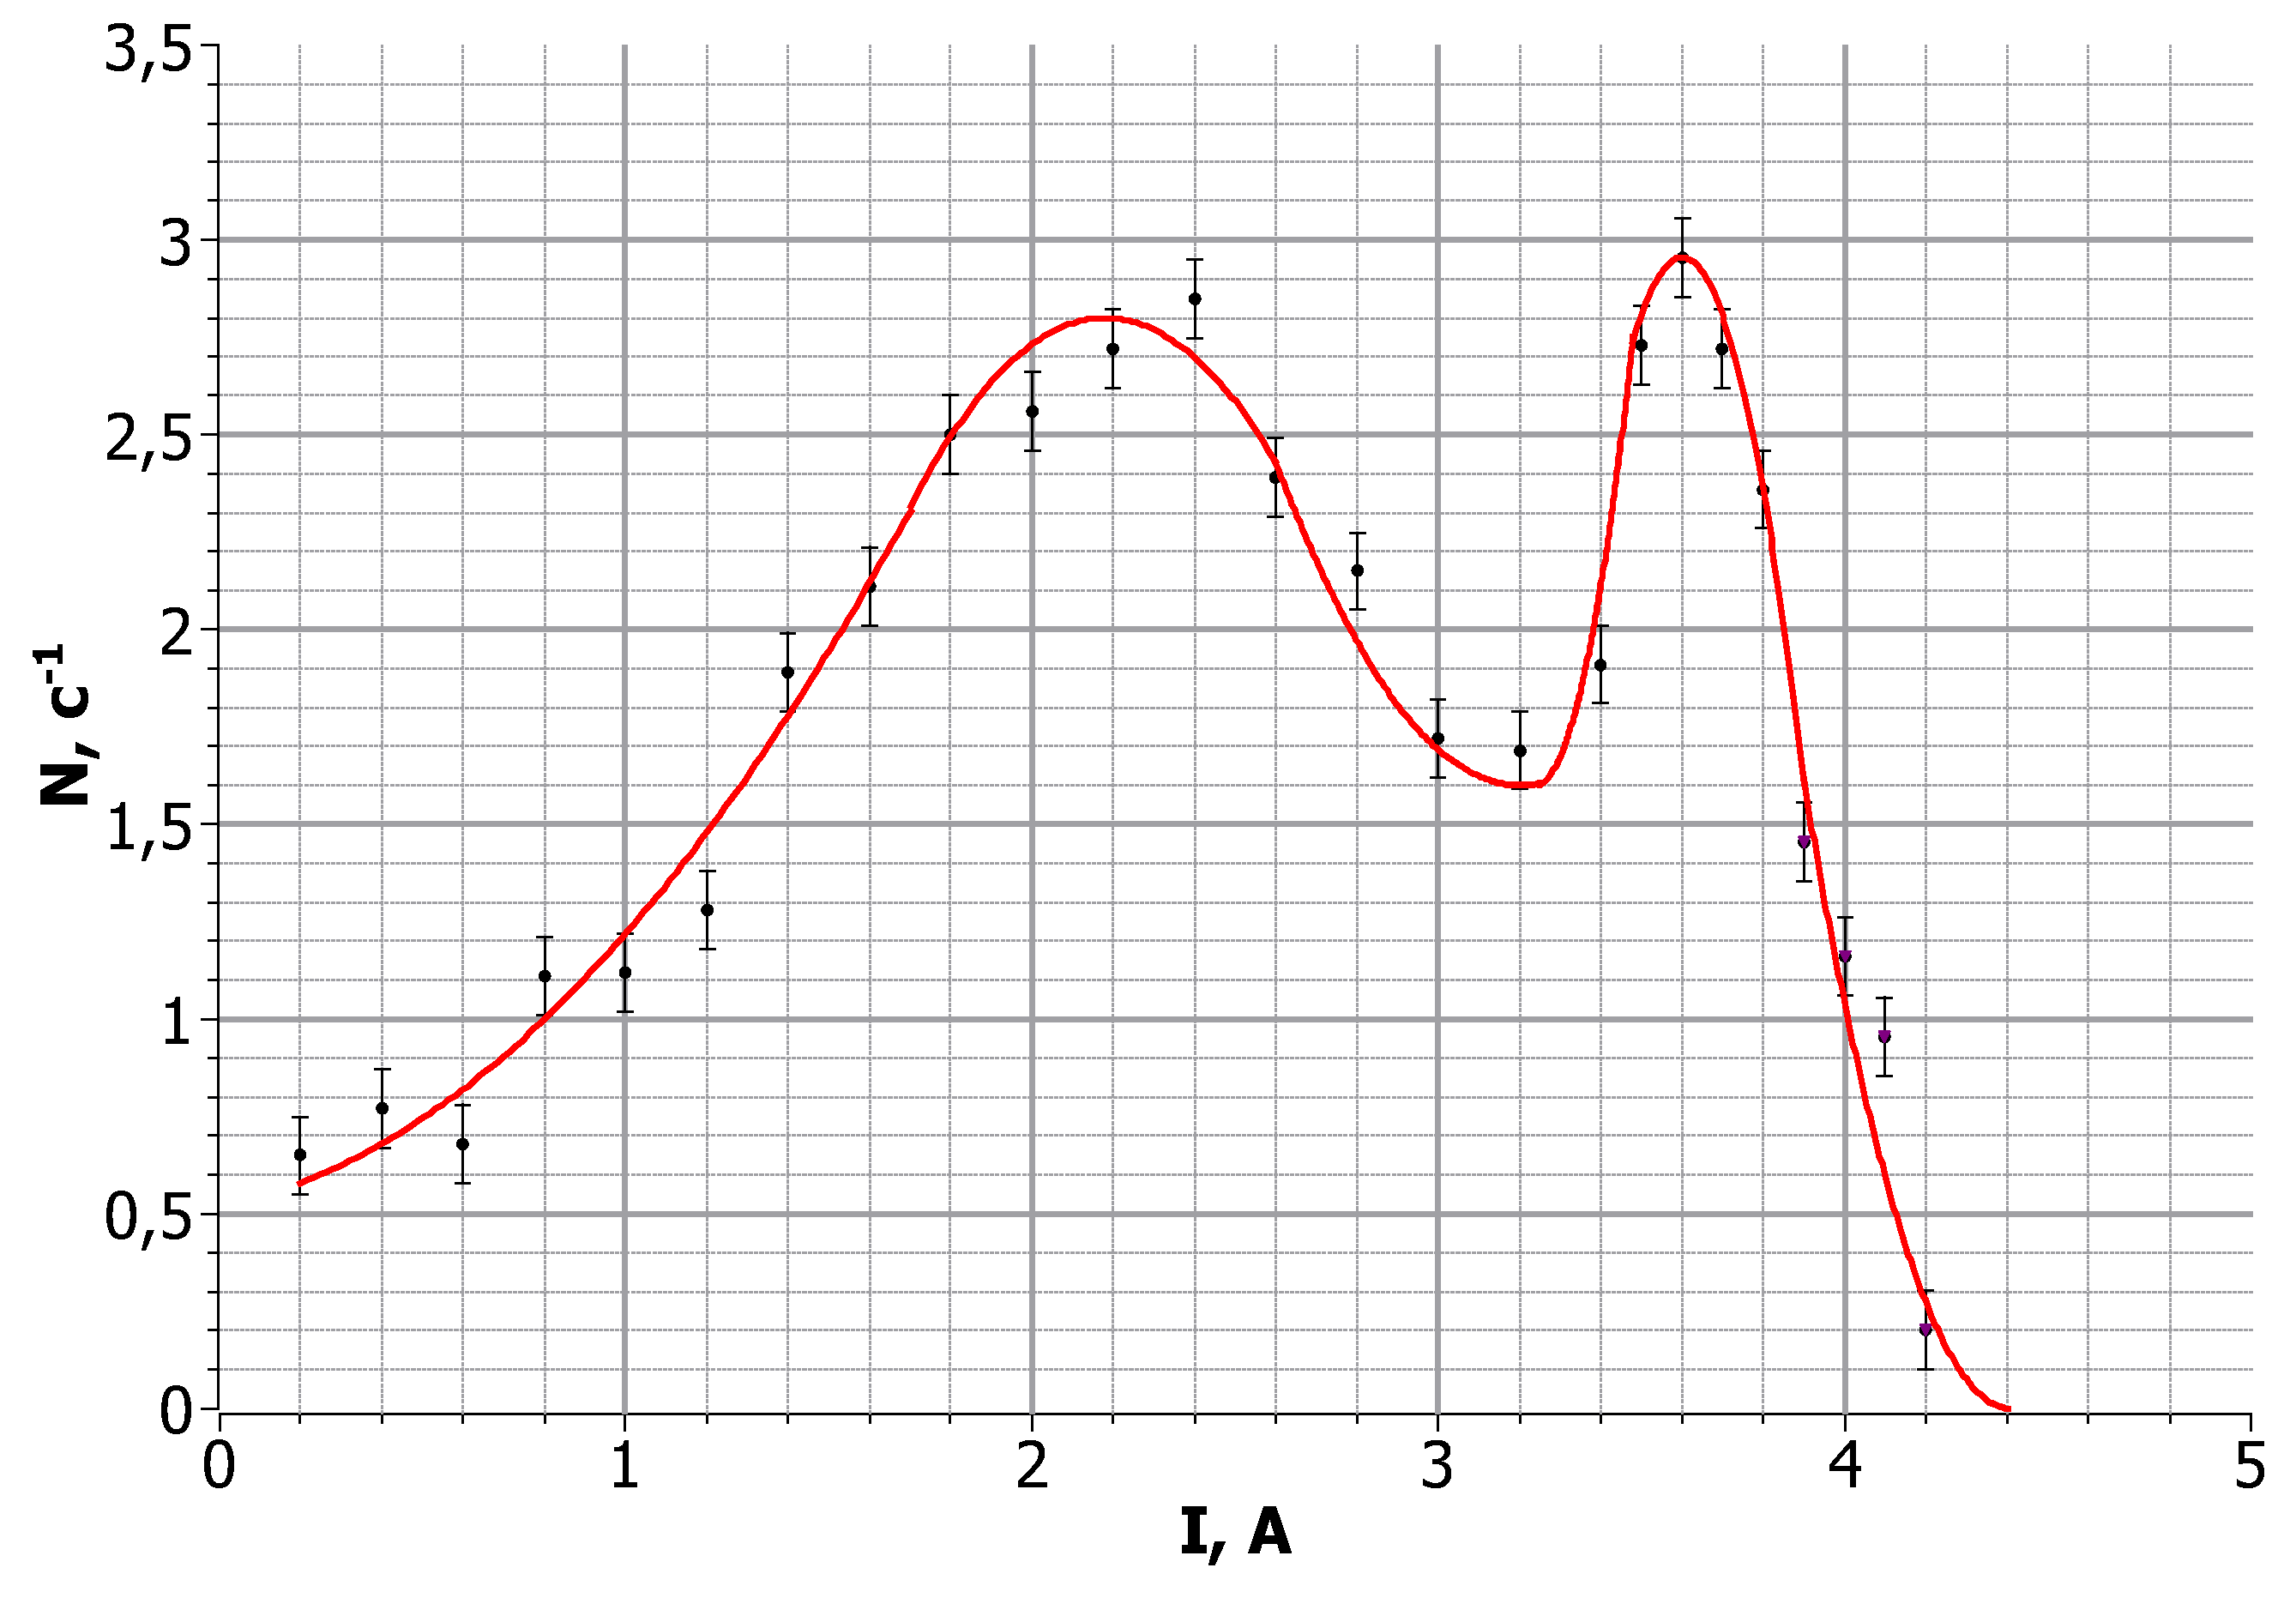
\includegraphics[width=\linewidth]{Pictures/Spectre.pdf}
			\caption{$\beta$-спектр за вычетом фона}
		\end{figure}
		
		\item Измерим фон. В нашем случае он получился $N_\text{ф} = 0,929$ с$^{-1}$. Эту информацию тоже занесем в таблицу \ref{BetaParticles_ExpTable}. 
		
		\begin{table}[h!]
			\centering
				\begin{tabular}{|l|l|l|}
					\hline
					\multicolumn{1}{|r|}{$I$, А} & \multicolumn{1}{r|}{$N$ с$^{-1}$} & \multicolumn{1}{r|}{$N - N_\text{ф}$, с$^{-1}$} \\ \hline
					0,2                          & 1,579                             & 0,650                                           \\ \hline
					0,4                          & 1,699                             & 0,770                                           \\ \hline
					0,6                          & 1,609                             & 0,680                                           \\ \hline
					0,8                          & 2,039                             & 1,110                                           \\ \hline
					1,0                          & 2,049                             & 1,120                                           \\ \hline
					1,2                          & 2,209                             & 1,280                                           \\ \hline
					1,4                          & 2,819                             & 1,890                                           \\ \hline
					1,6                          & 3,039                             & 2,110                                           \\ \hline
					1,8                          & 3,429                             & 2,500                                           \\ \hline
					2,0                          & 3,489                             & 2,560                                           \\ \hline
					2,2                          & 3,649                             & 2,720                                           \\ \hline
					2,4                          & 3,779                             & 2,850                                           \\ \hline
					2,6                          & 3,319                             & 2,390                                           \\ \hline
					2,8                          & 3,079                             & 2,150                                           \\ \hline
					3,0                          & 2,649                             & 1,720                                           \\ \hline
					3,2                          & 2,619                             & 1,690                                           \\ \hline
					3,4                          & 2,839                             & 1,910                                           \\ \hline
					3,5                          & 3,659                             & 2,730                                           \\ \hline
					3,6                          & 3,884                             & 2,955                                           \\ \hline
					3,7                          & 3,649                             & 2,720                                           \\ \hline
					3,8                          & 3,289                             & 2,360                                           \\ \hline
					3,9                          & 2,382                             & 1,453                                           \\ \hline
					4,0                          & 2,089                             & 1,160                                           \\ \hline
					4,1                          & 1,882                             & 0,953                                           \\ \hline
					4,2                          & 1,130                             & 0,201                                           \\ \hline
				\end{tabular}
			\caption{Экспериментальные данные}
			\label{BetaParticles_ExpTable}
		\end{table}
	
	
		\item По конверсионному пику определим константу пропорциональности $k$ из уравнения \eqref{BetaParticles_pkI}. Величина произведения импульса конверсионного электрона на скорость света равна 1013,5 кэВ. Откуда:
		\begin{equation*}
			k = 281,5 \cdot \frac{1}{c}\; \frac{\text{кэВ}}{\text{A}},
		\end{equation*}
	 	\noindent где $c$ -- это скорость света, а не секунды.
	 	
	 	\item Теперь, зная эту калибровочную константу, построим график Ферми-Кюри, то есть зависимость величины $\frac{\sqrt{N}}{p^{3/2}}$ от энергии электрона $E$. Из него, по пересечению с осью абсцисс можно определить максимальную энергию $\beta$-частиц.
		
		
		% Please add the following required packages to your document preamble:
		% \usepackage{graphicx}
		\begin{table}[h!]
			\centering
			\resizebox{0.9\columnwidth}{!}{%
				\begin{tabular}{|r|r|r|r|r|r|}
					\hline
					\multicolumn{1}{|r|}{$I$, А} & \multicolumn{1}{r|}{$N$, с$^{-1}$} & \multicolumn{1}{r|}{$N - N_\text{ф}$, с$^{-1}$} & \multicolumn{1}{r|}{$p = k \cdot I$, кэВ/c} & \multicolumn{1}{r|}{$\sqrt{N}/p^{3/2}$, $c^{3/2} \cdot 10^{-6}$ сек$^{-1/2} \cdot$ кэВ$^{-3/2}$} & \multicolumn{1}{r|}{$E$, кэВ} \\ \hline
					0,2                          & 1,579                              & 0,650                                          & 56,3                                        & 1908,51                                                                                          & 3,09                          \\ \hline
					0,4                          & 1,699                              & 0,770                                          & 112,6                                       & 734,41                                                                                           & 12,26                         \\ \hline
					0,6                          & 1,609                              & 0,680                                          & 168,9                                       & 375,67                                                                                           & 27,19                         \\ \hline
					0,8                          & 2,039                              & 1,110                                          & 225,2                                       & 311,75                                                                                           & 47,42                         \\ \hline
					1,0                          & 2,049                              & 1,120                                          & 281,5                                       & 224,07                                                                                           & 72,41                         \\ \hline
					1,2                          & 2,209                              & 1,280                                          & 337,8                                       & 182,23                                                                                           & 101,56                        \\ \hline
					1,4                          & 2,819                              & 1,890                                          & 394,1                                       & 175,72                                                                                           & 134,32                        \\ \hline
					1,6                          & 3,039                              & 2,110                                          & 450,4                                       & 151,97                                                                                           & 170,16                        \\ \hline
					1,8                          & 3,429                              & 2,500                                           & 506,7                                       & 138,63                                                                                           & 208,63                        \\ \hline
					2,0                          & 3,489                              & 2,560                                          & 563,0                                       & 119,77                                                                                           & 249,32                        \\ \hline
					2,2                          & 3,649                              & 2,720                                          & 619,3                                       & 107,01                                                                                           & 291,90                        \\ \hline
					2,4                          & 3,779                              & 2,850                                          & 675,6                                       & 96,14                                                                                            & 336,09                        \\ \hline
					2,6                          & 3,319                              & 2,390                                          & 731,9                                       & 78,08                                                                                           & 381,64                        \\ \hline
					2,8                          & 3,079                              & 2,150                                          & 788,2                                       & 66,26                                                                                            & 428,35                        \\ \hline
					3,0                          & 2,649                              & 1,720                                          & 844,5                                       & 53,44                                                                                            & 476,07                        \\ \hline
					3,2                          & 2,619                              & 1,690                                          & 900,8                                       & 48,08                                                                                            & 524,65                        \\ \hline
					3,4                          & 2,839                              & 1,910                                          & 957,1                                       & 46,67                                                                                            & 573,97                        \\ \hline
					3,5                          & 3,659                              & 2,730                                          & 985,3                                       & 53,43                                                                                            & 598,88                        \\ \hline
					3,6                          & 3,884                              & 2,955                                          & 1013,4                                      & 53,29                                                                                            & 623,95                        \\ \hline
					3,7                          & 3,649                              & 2,720                                          & 1041,6                                      & 49,06                                                                                            & 649,15                        \\ \hline
					3,8                          & 3,289                              & 2,360                                          & 1069,7                                      & 43,91                                                                                            & 674,49                        \\ \hline
					3,9                          & 2,382                              & 1,453                                          & 1097,9                                      & 33,14                                                                                            & 699,95                        \\ \hline
					4,0                          & 2,089                              & 1,160                                          & 1126,0                                      & 28,51                                                                                            & 725,53                        \\ \hline
					4,1                          & 1,882                              & 0,953                                          & 1154,2                                      & 24,90                                                                                            & 751,21                        \\ \hline
					4,2                          & 1,130                              & 0,201                                          & 1182,3                                      & 11,03                                                                                            & 777,00                        \\ \hline
				\end{tabular}%
			}
		\end{table}
	
		\begin{figure}[h!]
			\centering
			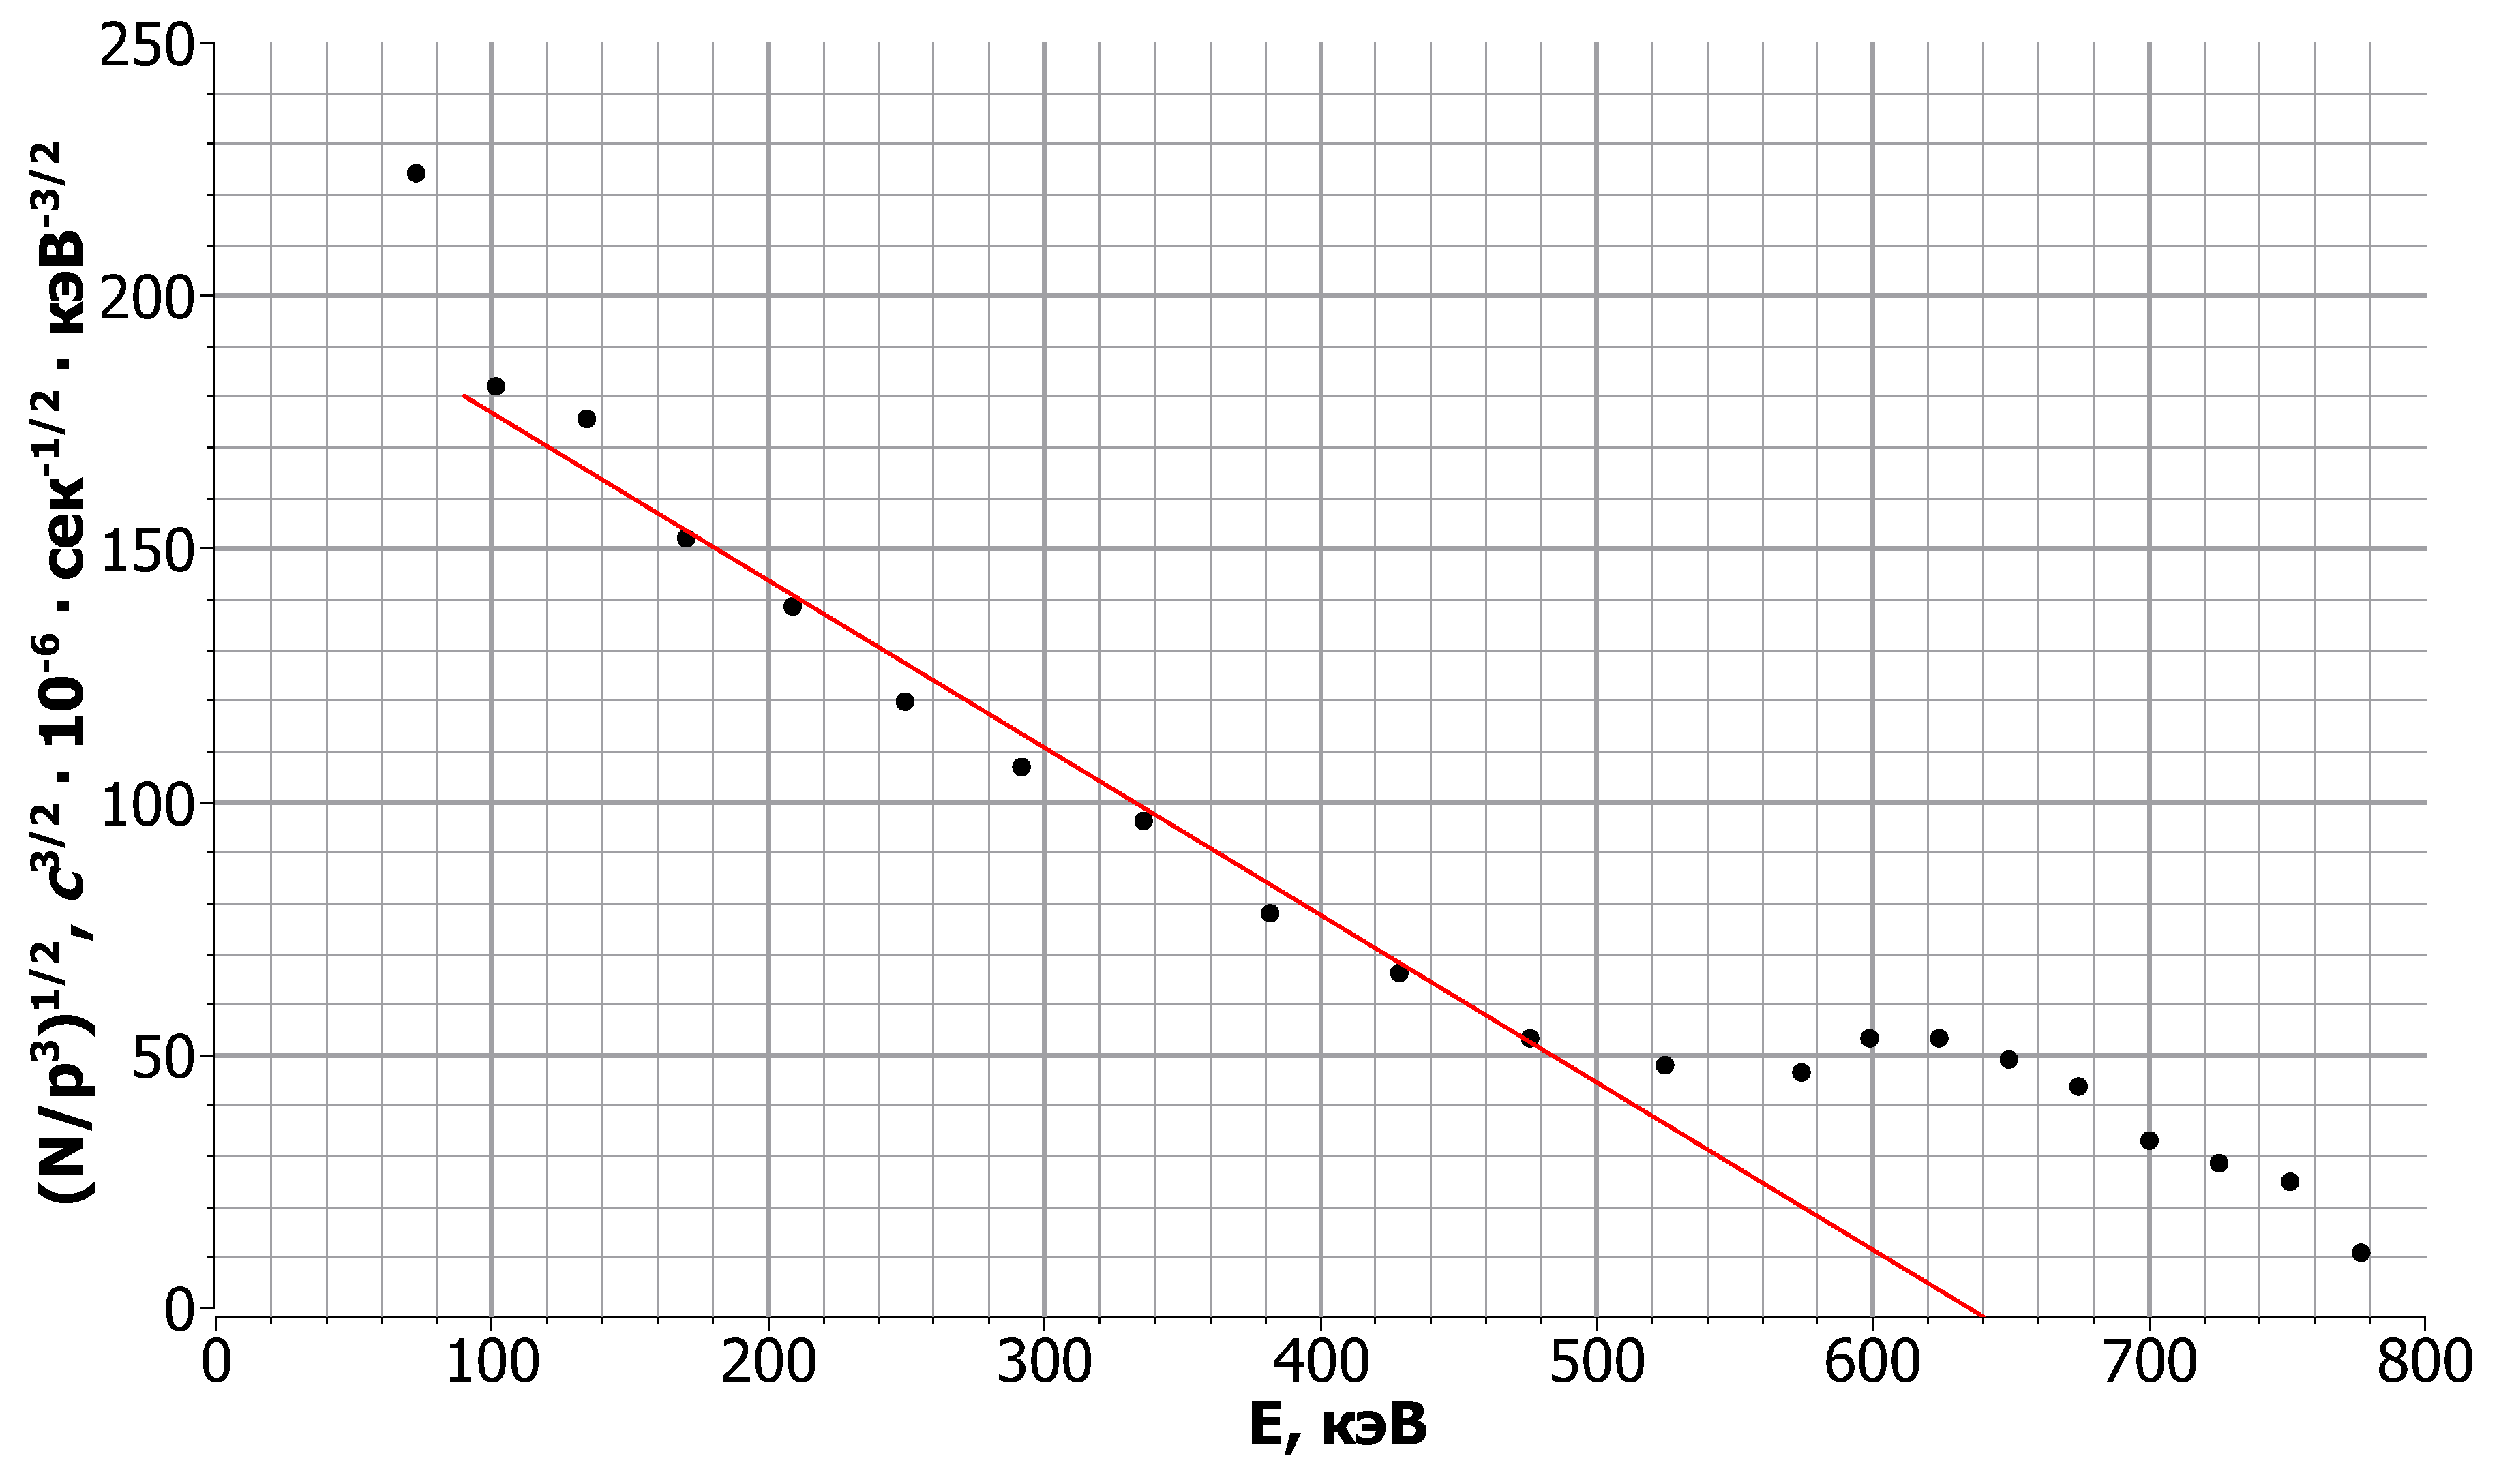
\includegraphics[width=\linewidth]{Pictures/jopa(E).pdf}
			\caption{График Ферми-Кюри}
		\end{figure}
	
		Для построения графика не использовались первые 4 точки, поскольку они давали слишком большие значения по ординате из-за чего главную часть графика не было хорошо видно.
		
		Также, мы видим, что сам график хоть и напоминает прямую, однако все же он не линеен. Именно поэтому строим аппроксимирующую прямую лишь по линейному участку.
		
		Получаем следующие коэффициенты для аппроксимации прямой вида $y = Ax + B$:
		\begin{itemize}
			\item $A = (-0,33 \pm 0,02)$ $c^{3/2} \cdot 10^{-6}$ сек$^{-1/2} \cdot$ кэВ$^{-5/2}$
			
			\item $B = (210 \pm 5)$ $c^{3/2} \cdot 10^{-6}$ сек$^{-1/2} \cdot$ кэВ$^{-3/2}$
		\end{itemize}
	
		Максимальная энергия $\beta$-частиц определяется пересечением прямой с осью абсцисс:
		\begin{equation*}
			E_\text{max} = -\frac{B}{A}
		\end{equation*}
		\begin{equation*}
			\boxed{E_\text{max} = (640 \pm 30) \text{ кэВ}}
		\end{equation*}
		
		Относительная погрешность составляет $\thicksim 5\%$.
		
		В принципе, значение недалеко от правды: $E_\text{max}^\text{истин} \simeq 634 \text{ кэВ}$.
	\end{enumerate}
	
	
	\tocsection{Вывод}
	В данной работе мы исследовали спектр $\beta$-частиц при распаде цезия $^{137}$Cs. Также, была определена максимальная энергия $\beta$-частиц при данном распаде: $E_\text{max} = (640 \pm 30)$ кэВ. Относительная погрешность составляет $\thicksim 5\%$. Причем истинное значение находится близко к найденному нами: $E_\text{max}^\text{истин} \simeq 634$ кэВ. Хоть ошибки и есть, но достаточно малы.
	
\end{document}